% !TEX root = ../Thesis.tex

\section{Planning}
\label{sec:planning}

\subsection{Original planning}
In the original planning \citepr{plan}, two kinds of deadlines have been identified: development iterations and project phases.
The project phase deliveries were scheduled as follows:
 \begin{enumerate}
	\item Phase 2 - Task allocation and Project plan			-- 	2014-11-13
 	\begin{enumerate}
		\item Delivery of the detailed project plan 			
		\item Detailed allocation of tasks within the project team 
	\end {enumerate}
	\item Phase 3a - Domains \& Techniques					-- 	2014-12-17
 	\begin{enumerate}
		\item Delivery of scientific article by Daniel Schiavini
		\item Delivery of scientific article by Maarten Baertsoen
	\end {enumerate}
 	\item Phase 3b - Research context
 	\begin{enumerate}
		\item Detailed report of the `research context'  		-- 	2015-04-29
	\end {enumerate}
 	\item Phase 3c - Design \& implementation				-- Last iteration on 2015-04-08 (see below)
 	\begin{enumerate}
		\item Analysis \& design documents
		\item Test report
		\item Source code
	\end {enumerate}
 	\item Phase 3d - Project documentation					-- 	2015-05-04
 	\begin{enumerate}
		\item Project documentation document	
	\end {enumerate}
	\item Phase 4 - Project closure and final project presentation
 	\begin{enumerate}
		\item Project essay							-- 	2015-05-20
		\item Project presentation						-- 	date to be jointly determined, final due date 29/05/2014
	\end {enumerate}
\end {enumerate}
%
Besides, the iteration deliveries were planned on the following dates:
\begin{longtable}{|l|l|}\hline
    \textbf{Date} & \textbf{Deliverable (s)} \\\hline
	\endhead
    2015-02-04 & Delivery iteration 1\\\hline
    2015-02-25 & Delivery iteration 2\\\hline
    2015-03-18 & Delivery iteration 3\\\hline
    2015-04-08 & Delivery iteration 4\\\hline
  \caption{Realization milestones}
  \label{tab:realization-milestones}
\end{longtable}


\subsection{Planning evaluation}
Just after delivering the project planning, one thing was clear for us: we planned too much.
During the planning phase, we took both too long to deliver the document, but we also spent too many hours doing so.
We also promised a more formal approach than it was requested by the customer and supervisor.

Happily though, we had kept a good track of the time spent in the project from the beginning on.
Although we spent almost 150 hours in the planning and preparation phase (expected: 40 hours), we then had gathered so much information about the project, that we could immediately begin with the implementation.

The planned amount of 15 hours of work per week came to be too much after some changes in our personal life (e.g. new house, new work, sickness).
We were hardly being able to work 10 hours per week in the project.
Therefore, we could not reach most self-inflicted deadlines.
In \autoref{tab:delivery-dates} we summarize the planned and actual delivery dates.%
%
\begin{longtable}{|l|l|p{6cm}|}\hline
    \textbf{Planned date} & \textbf{Phase} & \textbf{Delivered on} \\\hline
	\endhead
    2014-11-13 & Phase 2: Project plan  & 2014-11-29 (+16 days)\\\hline
    2014-12-17 & Phase 3a: Domains \& Techniques  & 2014-12-16 (Daniel, -1 day) and\newline
                                                    2015-02-05 (Maarten, +50 days) \\\hline
    2015-04-29 & Phase 3b: Research context  & 2015-06-11 (+43 days) \\\hline
    2015-04-08 & Phase 3c: Design \& implementation  & 2015-06-08 (+61 days) \\\hline
    2015-05-04 & Phase 3d: Project documentation  & 2015-06-08 (+35 days) \\\hline
    2015-05-20 & Phase 4: Thesis  & 2015-06-16 (+27 days) \\\hline
    2015-05-29 & Phase 4: Project presentation  & 2015-06-30 (+32 days) \\\hline
  \caption{Planned and actual delivery dates}
  \label{tab:delivery-dates}
\end{longtable}%
%
The delay in the planning was communicated clearly with the supervisor and customer.
Since both were understanding and were not in a hurry to finish the project, just moving the deadlines was not a problem.

We had less time available than expected for the project; however, the time spent was in our opinion very fruitful and efficient.
Since we believe we managed expectations well, the delay was not an issue after all.
We also could not have known beforehand that our personal lives were going to change.
In \autoref{fig:hour-statistics} we show some relevant statistics about the time spent in the project.

Our evaluation of the planning is thus that it was well done, though extensive.
%
\begin{figure}[htb!]
	\centering
	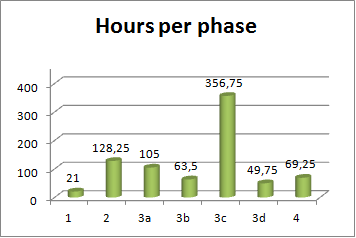
\includegraphics[width=0.45\textwidth]{Figures/HoursPerPhase}
	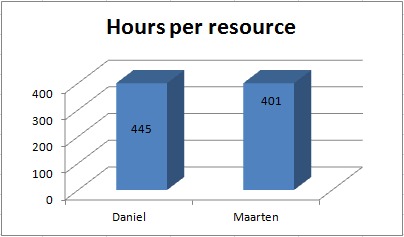
\includegraphics[width=0.45\textwidth]{Figures/HoursPerResource}
	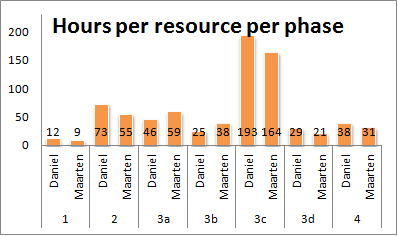
\includegraphics[width=0.55\textwidth]{Figures/HoursPerResourcePerPhase}
	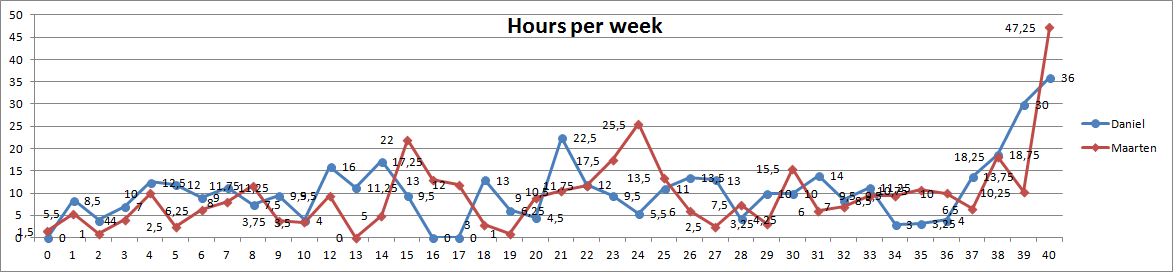
\includegraphics[width=1.00\textwidth]{Figures/HoursPerWeek}
	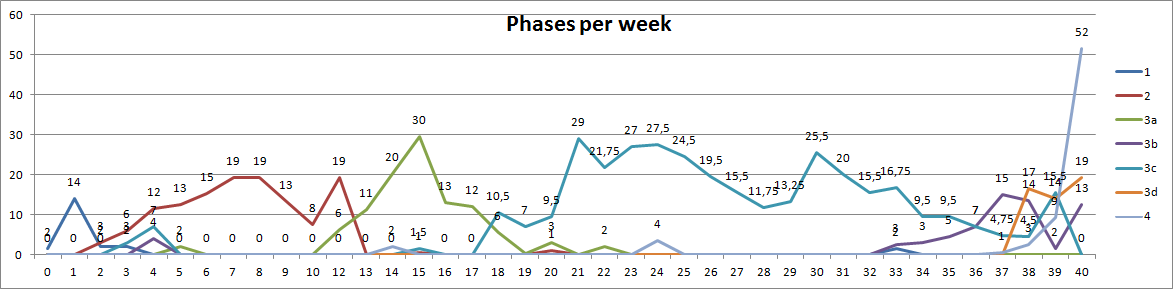
\includegraphics[width=1.00\textwidth]{Figures/HoursPerPhasePerWeek}
	\caption{Some relevant statistics about the time spent in the project.
%    TODO: Update these figures when done.
     }
	\label{fig:hour-statistics}
\end{figure}
